\documentclass[a4paper,11pt]{article}
\usepackage[english]{babel}
\usepackage[T1]{fontenc}
\usepackage{fancyhdr}
\usepackage{graphicx}
\usepackage{caption}
\usepackage{subcaption}
\usepackage{a4wide}
\usepackage{numprint}
\usepackage{url}
\usepackage{cite}
\usepackage{multirow}
\usepackage{moreverb}
\usepackage{lastpage}
\usepackage{enumerate}
\pagestyle{fancy}

\author{Viktor Collin \\ <\url{vcollin@kth.se}> \\ 19880316-0277 \and Simon \"{O}sterman \\ <\url{simost@kth.se}> \\ 19880205-0156}
\title{\textbf{DH2323 Computer Graphics with Interaction \\ Lab 2 : Raytracer}}

\fancyhead[L]{\textbf{DH2323 : Lab 2} }
\fancyhead[R]{Viktor Collin \& Simon \"{O}sterman : Page \thepage }
\fancyfoot{}{}

\begin{document}
\maketitle
\begin{center}
Total pages: \pageref{LastPage}
\end{center}
\thispagestyle{empty}

\clearpage
\setcounter{page}{1}
\section{Introduction}
The purpose of this lab is to learn how to build a raytracer and use it to render an image of a 3D environment that consists of triangular shapes. The lab also includes light models, shading and camera movement. 
\section{Assignment}
The assignment is to implement a raytracer which can create images given a 3D-model by tracing the rays reaching a simulated camera. The implementation should be done in several steps, each with new functionality or other improvements. The final implementation should include a mobile camera, simulated light-sources as well as light reflection for diffuse surfaces.
\section{Method}
\subsection{First implementation}
As a first step we built our raytracer to send a ray through each pixel on the screen and finding the closes intersection with the predefined model of the room. Next, it renders that pixel to be the color of the intersected shape. If the ray did not hit any shape, we render the pixel to be black. See the output of this in figure \ref{fig1}.

\subsection{Camera movement}
Next step is to implement an interactive environment were the user with the help of the keyboard is able to move and rotate the camera. Rotations is implemented by increasing or decreasing an angle and then updating the rotation matrix \verb|R|. Movement in the forward and backward directions is then done by multiplying \verb|R| with the movement speed in the \verb|z|-direction. The rays sent through each pixel is then sent in the direction of the camera.

\subsection{Direct light}
To introduce shading we placed a light source in the ceiling of the room. When the ray from the camera hit a shape and the normal of that shape is facing away from the light, then there is no light that hits the surface. See the output of this in figure \ref{fig2}. We also send a new ray from the intersection point towards the light source to see if there was an object shadowing that pixel. If so, the pixel gets painted black, otherwise the amount of light is calculated based on the distance from the light. At first, this implementation did not take into consideration the color of the shape that was hit by the first ray. See the output of the shading in figure \ref{fig3}.
We also implemented the possibility for the user to move the light source in a similar way as moving the camera but instead of rotating, it moves in the \verb|x|-direction.
To take into consideration the colors of the boxes and walls, we multiply the color with the direct light. See the output of this in figure \ref{fig4}

\subsection{Indirect light}
Instead of making the light bouncing and defusing on each surface which is a complex task, we just overlay the direct light with a uniform light for all pixels. This is a much simpler way and the result is reasonably realistic. We just add a constant light to the direct light before the color computation. The result can be seen in figure \ref{fig5}. 

\section{Result}
This lab was a bit more complex then the first one. We had the same trouble with the comparisons of floating point number and integers eg. float == 0 is often not true due to bad precision of floating point numbers. This gave us some strange behaviors in the beginning. The quality of the final output could be improved even further using anti-aliasing to get smoother edges. However, our rendering time is already 20s and implementing this would make the program run about four times slower. 

\begin{figure}[h!]
	\centering	
	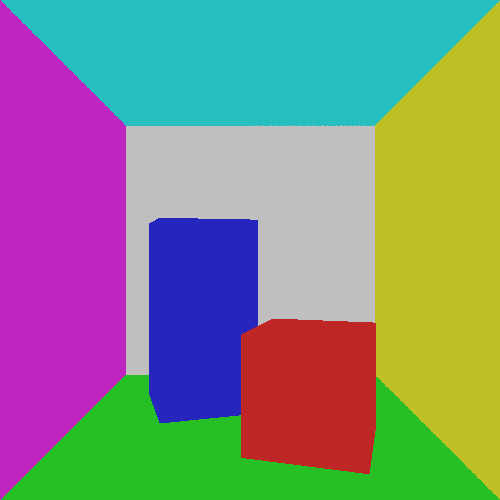
\includegraphics[width=0.45\linewidth]{screenshot1.png}
	\caption{Output from first run without lighting}
	\label{fig1}
\end{figure}

As can be seen above, a picture without lighting is ridiculously far from a realistic looking pictures but as soon as lighting and shadows are introduced it gets better real fast. It was fun to see the picture evolving for each completed implementation step. 

\begin{figure}[h!]
	\centering
	\begin{subfigure}[h]{0.3\linewidth}
		\centering
		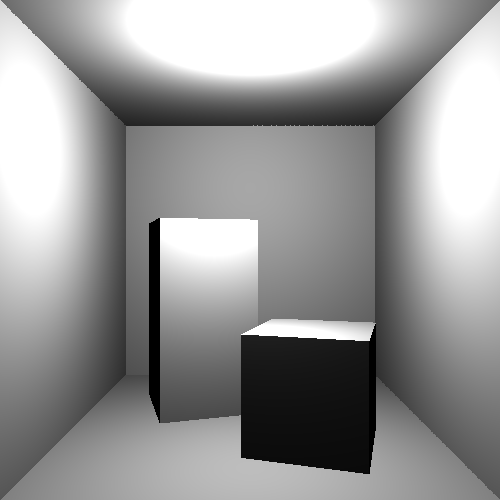
\includegraphics[width=\linewidth]{screenshot2.png}
		\caption{Facing away from light}
		\label{fig2}
	\end{subfigure}
	\begin{subfigure}[h!]{0.3\linewidth}
		\centering
		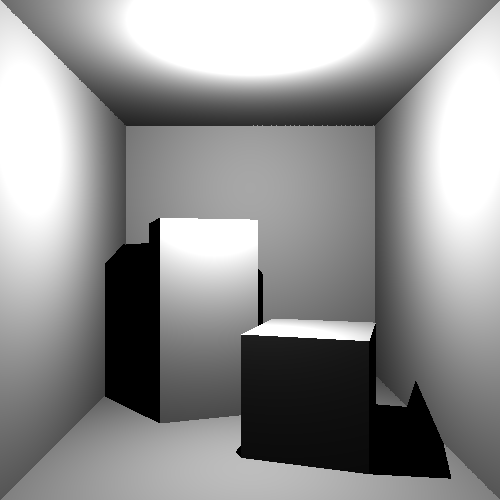
\includegraphics[width=\linewidth]{screenshot25.png}
		\caption{With shadows}
		\label{fig3}
	\end{subfigure}
	\begin{subfigure}[h!]{0.3\linewidth}
		\centering
		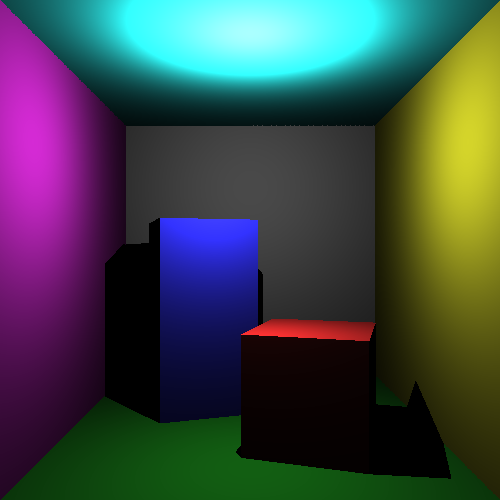
\includegraphics[width=\linewidth]{screenshot3.png}
		\caption{With shadows and colors}
		\label{fig4}
	\end{subfigure}
	\caption{Progress of the direct light model}
\end{figure}

\begin{figure}[h!]
	\centering	
	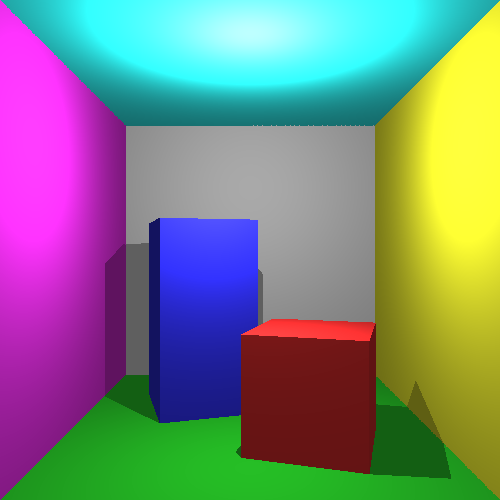
\includegraphics[width=0.45\linewidth]{screenshot4.png}
	\caption{Output from the finished program}
	\label{fig5}
\end{figure}



\end{document}
